\section{Results}
\label{sec:results}

The retrieval comparison and the threshold sweep make no model call and are complete. The end-to-end evaluation had 132 of its 240 planned answers when this version was written (2026-11-16): the two gated systems and the \code{no_rag} baseline are complete on the default model.

\subsection{Retrieval and gate comparison}
\label{sec:retrieval-results}

\begin{table}[htbp]
\centering
\caption{Retrieval and gate comparison, with no LLM call (from \texttt{results/retrieval.csv}). Hit rates and context precision are on the 20 answerable questions; auroc, margin and gap\_share separate them from the 10 out-of-corpus ones, the heldout columns from the 10 held-out ones. BM25 is the keyword baseline. \emph{+name} rows reorder the 20 fused candidates with a cross-encoder; \emph{\_gate} rows keep the hybrid passages and use the cross-encoder score only for the refusal gate. The margin is in the units of each score (cosine, BM25 score, cross-encoder logit or probability); gap\_share divides it by the score range.}
\label{tab:retrieval}
\resizebox{\linewidth}{!}{%
\begin{tabular}{llrrrrrrrrr}
\toprule
Retriever & Used by & hit\_rate & page\_hit\_rate & context\_precision & auroc & margin & gap\_share & heldout\_auroc & heldout\_margin & mean\_latency\_ms \\
\midrule
dense & rag\_dense & 0.95 & 0.8 & 0.857 & 1.0 & 0.0357 & 0.074 & 0.95 & -0.0806 & 144 \\
bm25 & bm25\_rag (baseline) & 1.0 & 0.95 & 0.932 & 0.945 & -5.8951 & -0.157 & 0.635 & -24.8051 & 9 \\
hybrid & rag\_hybrid, rag\_rerank & 1.0 & 0.9 & 0.911 & 1.0 & 0.0357 & 0.074 & 0.95 & -0.0806 & 158 \\
hybrid+medcpt & -- & 0.95 & 0.8 & 0.889 & 0.995 & -0.0001 & -0.0 & 0.975 & -0.0002 & 13089 \\
hybrid+medcpt\_gate & -- & 1.0 & 0.9 & 0.911 & 1.0 & 0.2224 & 0.222 & 0.97 & -0.0013 & 2714 \\
hybrid+bge & -- & 1.0 & 0.95 & 0.908 & 1.0 & 0.0633 & 0.064 & 1.0 & 0.0182 & 49628 \\
hybrid+bge\_gate & -- & 1.0 & 0.9 & 0.911 & 1.0 & 0.0283 & 0.028 & 0.995 & -0.0169 & 10235 \\
hybrid+minilm & -- & 0.95 & 0.9 & 0.906 & 1.0 & 3.5874 & 0.19 & 0.96 & -3.545 & 2095 \\
hybrid+minilm\_gate & rag\_rerank (gate) & 1.0 & 0.9 & 0.911 & 1.0 & 3.5874 & 0.187 & 0.955 & -3.545 & 597 \\
\bottomrule
\end{tabular}}
\end{table}


In Table~\ref{tab:retrieval}, hit rate, page hit rate (the evidence page is among the 5 passages) and context precision are measured on the 20 answerable questions. The last columns measure how well a gate's score separates answerable from out-of-corpus questions: \emph{auroc} is the share of (answerable, out-of-corpus) pairs in which the answerable one scores higher; \emph{margin} is the lowest answerable score minus the highest out-of-corpus score, positive when one threshold separates them all.

\paragraph{Passages.} The hybrid passages find the expected document for every answerable question (hit rate 1.0) and the evidence page for 18 of 20 (page hit rate 0.90), against 0.95 and 0.80 for dense retrieval alone. BM25 alone does better still on these questions: page hit rate 0.95 and context precision 0.932. A likely reason is that the answerable questions were written from passages of the corpus, so they often share their words, which favours a keyword ranking. For example, BM25 finds the evidence page of A07 (the single dose of primaquine) where dense retrieval does not (\code{results/retrieval_questions.csv}). Reordering the fused candidates with a cross-encoder did not pay off: MedCPT found fewer evidence pages (0.80), MiniLM as many (0.90), and bge-reranker-v2-m3 one more (0.95) at about 50 seconds per question on our CPU. So the cross-encoder only gates.

\paragraph{Gate scores.} The dense similarity ranks every answerable question above every out-of-corpus one (auroc 1.0), but the margin is small: 0.0357, between A04 (0.6235, the lowest answerable) and O06 (0.5878, the highest out-of-corpus). The BM25 score cannot gate (auroc 0.945, negative margin): it grows with the number and rarity of the question's terms, not only with relevance. The three cross-encoders used as gates also reach auroc 1.0 on the 30 questions, so the ranking does not separate them. What separates them is where the model's own 0.5 boundary falls. Only MiniLM answers all 20 answerable questions and refuses all 10 out-of-corpus ones at 0.5: its lowest answerable score is 0.870 and its highest out-of-corpus score is 0.156 (O06, the isotretinoin question). MedCPT lets ``Who painted the Mona Lisa?'' through (0.78), and bge-reranker-v2-m3 the multiple sclerosis question (0.85). MiniLM is also the fastest (0.6 seconds per question with all 5 passages; about 0.3 seconds for an answerable question in the system, which stops early). We chose it as the gate.

This choice was made on the out-of-corpus questions, so the separation is not an independent test. The held-out questions N01 to N10, used to choose nothing, give that test, and the gate does worse on it. Against the answerable questions, the MiniLM gate score reaches auroc 0.955, not 1.0, and five of the ten reach its 0.5 boundary: N02 (0.702), N04 (0.950), N06 (0.977), N08 (0.996) and N10 (0.810). The dense similarity lets three through 0.6 (N06, N08 and N10; auroc 0.95). Their passages match the subject but lack the fact asked. Only bge-reranker-v2-m3, scoring the passages it reorders, ranks every answerable question above every held-out one (auroc 1.0, margin 0.018), at about 50 seconds per question. In the evaluation, the model's own refusal caught every held-out question that passed a gate (Table~\ref{tab:reasons}).

\subsection{Threshold sweep}
\label{sec:sweep}

\begin{table}[htbp]
\centering
\caption{Threshold sweep of the dense similarity gate on the original 30 questions (from \texttt{results/threshold\_sweep.csv}). Balanced is the mean of the answer rate on A01--A20 and the refusal rate on O01--O10. The lowest threshold, which refuses almost nothing, plays the role of a system without a gate.}
\label{tab:sweep}
{%
\begin{tabular}{rrrrl}
\toprule
Threshold & Answer rate & Refusal rate & Balanced & Note \\
\midrule
0.3 & 1.0 & 0.0 & 0.5 &  \\
0.35 & 1.0 & 0.1 & 0.55 &  \\
0.4 & 1.0 & 0.2 & 0.6 &  \\
0.45 & 1.0 & 0.3 & 0.65 &  \\
0.5 & 1.0 & 0.3 & 0.65 &  \\
0.55 & 1.0 & 0.7 & 0.85 &  \\
0.6 & 1.0 & 1.0 & 1.0 & best balanced \\
0.65 & 0.95 & 1.0 & 0.975 &  \\
0.7 & 0.65 & 1.0 & 0.825 &  \\
0.75 & 0.25 & 1.0 & 0.625 &  \\
0.8 & 0.1 & 1.0 & 0.55 &  \\
\bottomrule
\end{tabular}}
\end{table}

\begin{figure}[htbp]
\centering
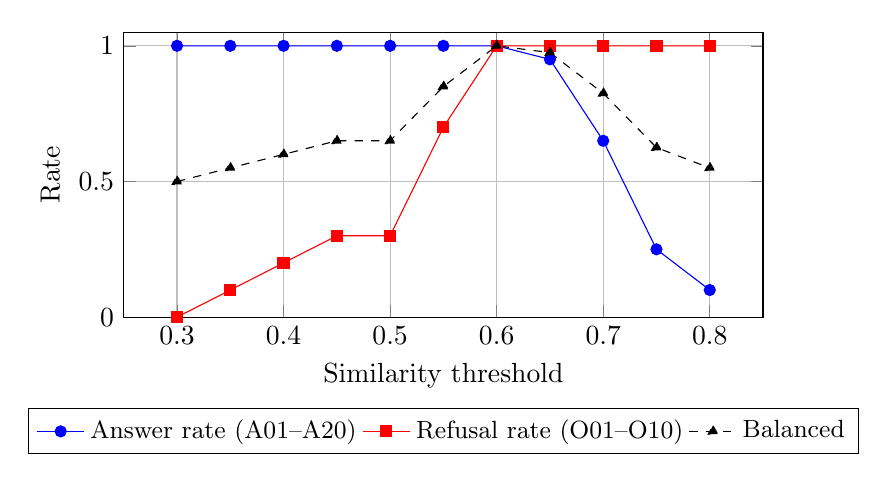
\begin{tikzpicture}
\begin{axis}[width=0.8\linewidth, height=5.2cm, xlabel={Similarity threshold}, ylabel={Rate}, ymin=0, ymax=1.05, grid=major, legend columns=3, legend style={at={(0.5,-0.32)}, anchor=north, font=\small}]
\addplot[blue, mark=*] coordinates {(0.3,1.0) (0.35,1.0) (0.4,1.0) (0.45,1.0) (0.5,1.0) (0.55,1.0) (0.6,1.0) (0.65,0.95) (0.7,0.65) (0.75,0.25) (0.8,0.1)};
\addlegendentry{Answer rate (A01--A20)}
\addplot[red, mark=square*] coordinates {(0.3,0.0) (0.35,0.1) (0.4,0.2) (0.45,0.3) (0.5,0.3) (0.55,0.7) (0.6,1.0) (0.65,1.0) (0.7,1.0) (0.75,1.0) (0.8,1.0)};
\addlegendentry{Refusal rate (O01--O10)}
\addplot[black, dashed, mark=triangle*] coordinates {(0.3,0.5) (0.35,0.55) (0.4,0.6) (0.45,0.65) (0.5,0.65) (0.55,0.85) (0.6,1.0) (0.65,0.975) (0.7,0.825) (0.75,0.625) (0.8,0.55)};
\addlegendentry{Balanced}
\end{axis}
\end{tikzpicture}
\caption{Answer rate, refusal rate and their mean (balanced) against the similarity threshold, on the original 30 questions (from \texttt{results/threshold\_sweep.csv}).}
\label{fig:sweep}
\end{figure}


The sweep (Table~\ref{tab:sweep}, Figure~\ref{fig:sweep}) applies thresholds from 0.30 to 0.80 to the best dense similarity of the original 30 questions. The brief's value, 0.60, is the only one with a balanced score of 1.0. At 0.55 the refusal rate drops to 0.70; at 0.65 the answer rate drops to 0.95, and to 0.25 at 0.75. A separating threshold must lie between 0.5878 and 0.6235, so the perfect score at 0.60 depends on two questions and is optimistic. We kept 0.60.

\subsection{End-to-end evaluation}
\label{sec:e2e}

\begin{table}[htbp]
\centering
\caption{Evaluation of each system and model (from \texttt{results/summary.csv}). \texttt{no\_rag} and \texttt{bm25\_rag} are the baselines. Answer: share of the answerable questions A01--A20 not refused. Ref.~O: share of the out-of-corpus questions O01--O10 refused. Ref.~N: share of the held-out questions N01--N10 refused. Hit: share of answerable questions with a passage from the expected source. CP: context precision. Faith.: faithfulness, with the number of judged answers in brackets. Lat.: mean seconds per answer. -- means no value.}
\label{tab:summary}
\resizebox{\linewidth}{!}{%
\begin{tabular}{lllrrrrrrrr}
\toprule
Role & System & Model & n & Answer & Ref. O & Ref. N & Hit & CP & Faith. & Lat. (s) \\
\midrule
baseline & \texttt{no\_rag} & nvidia/nemotron-3-ultra-550b-a55b:free & 6 & 1.0 & -- & -- & -- & -- & -- & 9.31 \\
RAG & \texttt{rag\_hybrid} & nvidia/nemotron-3-ultra-550b-a55b:free & 40 & 0.95 & 1.0 & 1.0 & 1.0 & 0.911 & 1.0 (19) & 5.18 \\
RAG & \texttt{rag\_rerank} & nvidia/nemotron-3-ultra-550b-a55b:free & 39 & 1.0 & 1.0 & 1.0 & 1.0 & 0.906 & 1.0 (19) & 6.03 \\
\bottomrule
\end{tabular}}
\end{table}

\begin{table}[htbp]
\centering
\caption{Outcome of each recorded answer, by system, model and question group (counted from \texttt{results/records.jsonl}). \texttt{no\_rag} and \texttt{bm25\_rag} are the baselines. Gate: refused before any model call. By model: the model wrote the refusal sentence. Uncited: the reply had no valid citation. Other: any other reason, such as no passage.}
\label{tab:reasons}
\resizebox{\linewidth}{!}{%
\begin{tabular}{lllrrrrrr}
\toprule
System & Model & Questions & n & Answered & Gate & By model & Uncited & Other \\
\midrule
\texttt{no\_rag} & nvidia/nemotron-3-ultra-550b-a55b:free & A01--A20 & 20 & 19 & 0 & 1 & 0 & 0 \\
\texttt{no\_rag} & nvidia/nemotron-3-ultra-550b-a55b:free & O01--O10 & 10 & 8 & 0 & 2 & 0 & 0 \\
\texttt{no\_rag} & nvidia/nemotron-3-ultra-550b-a55b:free & N01--N10 & 10 & 10 & 0 & 0 & 0 & 0 \\
\texttt{bm25\_rag} & nvidia/nemotron-3-ultra-550b-a55b:free & A01--A20 & 12 & 12 & 0 & 0 & 0 & 0 \\
\texttt{rag\_hybrid} & nvidia/nemotron-3-ultra-550b-a55b:free & A01--A20 & 20 & 19 & 0 & 1 & 0 & 0 \\
\texttt{rag\_hybrid} & nvidia/nemotron-3-ultra-550b-a55b:free & O01--O10 & 10 & 0 & 10 & 0 & 0 & 0 \\
\texttt{rag\_hybrid} & nvidia/nemotron-3-ultra-550b-a55b:free & N01--N10 & 10 & 0 & 7 & 3 & 0 & 0 \\
\texttt{rag\_rerank} & nvidia/nemotron-3-ultra-550b-a55b:free & A01--A20 & 20 & 19 & 0 & 1 & 0 & 0 \\
\texttt{rag\_rerank} & nvidia/nemotron-3-ultra-550b-a55b:free & O01--O10 & 10 & 0 & 10 & 0 & 0 & 0 \\
\texttt{rag\_rerank} & nvidia/nemotron-3-ultra-550b-a55b:free & N01--N10 & 10 & 0 & 5 & 5 & 0 & 0 \\
\bottomrule
\end{tabular}}
\end{table}


Table~\ref{tab:summary} is generated from \code{results/summary.csv} and Table~\ref{tab:reasons} from \code{results/records.jsonl}, as they stood after the second evaluation day (2026-11-16). \code{rag_rerank}, \code{rag_hybrid} and \code{no_rag} have their 40 answers; \code{bm25_rag} has 12 (A01 to A12); \code{rag_dense} and the second model have none. \TODO{after the last evaluation day: rerun \code{scripts/make_report_assets.py}, rebuild the PDF, and complete this subsection with the rows \code{bm25_rag}, \code{rag_dense} and the second model}

\paragraph{The gated systems.} On the default model, both gated systems refused all 10 out-of-corpus questions and all 10 held-out questions (refusal rate and held-out refusal rate 1.0), and answered 19 of the 20 answerable questions (answer rate 0.95): both refused A19 (Section~\ref{sec:errors}). Faithfulness is 1.0 over 19 judged answers for both, and context precision 0.911. The two rows are not independent: both systems retrieve the same passages, so the second reused the first one's answers and judge replies, and they differ only by their gate.

\paragraph{How the refusals happened.} Table~\ref{tab:reasons} shows that the refusal rates of 1.0 do not come from the gates alone. Every out-of-corpus question was stopped by the gate, with no model call. Of the held-out questions, the cosine gate of \code{rag_hybrid} stopped 7, and the model refused the other 3 after reading the passages. The cross-encoder gate of \code{rag_rerank} stopped only 5, and the model refused the other 5. On near-domain questions, the cross-encoder let more questions through than the cosine gate, the opposite of what the out-of-corpus questions suggested, and the prompt's instruction to refuse was the last defence for half of them (Section~\ref{sec:errors}).

\paragraph{The model alone.} \code{no_rag} answered 19 of the 20 answerable questions (it wrote the refusal sentence for A17), 8 of the 10 out-of-corpus questions and all 10 held-out questions: refusal rates of 0.2 and 0.0, against 1.0 and 1.0 for the gated systems. Its two out-of-corpus refusals are O08 and O10, two of the three questions that are not medical. Its prompt tells it to refuse only when it does not know, so these rates measure what the model believes it knows, not what the corpus holds, and none of its 37 answers names a passage a reader could check. Its answer rate of 0.95 equals that of the gated systems, but it measures that the model did not refuse, not that it was right: Section~\ref{sec:errors} compares its answers with the expected ones, and the human rating decides (Section~\ref{sec:human}).

\paragraph{The BM25 baseline.} \code{bm25_rag} has no gate. On its 12 recorded questions (A01 to A12) it answered all 12, with context precision 0.989 and faithfulness 1.0 over 12 judged answers. The questions where a missing gate matters, O01 to O10 and N01 to N10, are not recorded yet, and \code{rag_dense} has no record. \TODO{compare \code{rag_rerank} with \code{bm25_rag} and \code{rag_dense} on answer rate, refusal rates and human correctness once their rows are complete}

\paragraph{Latency.} The mean time per answer is 6.17 seconds for \code{rag_rerank}, 5.27 seconds for \code{rag_hybrid} and 8.11 seconds for \code{no_rag}, which calls the model for every question. A question stopped by a gate costs 0.1 to 0.7 seconds and a model call about 2 to 29 seconds. \code{rag_rerank} is slower mainly because its gate let 5 held-out questions reach the model, against 3. A reused answer counts the seconds of the original call.

\subsection{Model comparison}
\label{sec:models}

The brief's comparison of Llama~3 and GPT-4o-mini is replaced by \code{rag_rerank} on two free models, \code{nvidia/nemotron-3-ultra-550b-a55b:free} and \code{google/gemma-4-31b-it:free} (Section~\ref{sec:setup}). The second model runs last in the daily plan and has no record yet. \TODO{model comparison: read the two \code{rag_rerank} rows of Table~\ref{tab:summary}; compare answer rate, both refusal rates, faithfulness and latency, and note that the judge is the first model, which may favour it}

\subsection{Human evaluation}
\label{sec:human}

\begin{table}[htbp]
\centering
\caption{Human ratings from \code{results/human_rating_sheet.csv}, filled by the group members: share of correct answers (\code{correct_0_1}) and mean safety and clarity (1--5). \code{no_rag} and \code{bm25_rag} are the baselines.}
\label{tab:human}
\small
\begin{tabular}{@{}llrrrr@{}}
\toprule
Role & System (model) & Rated & Correct & Safety (1--5) & Clarity (1--5) \\
\midrule
baseline & \code{no_rag} & \TODO{} & \TODO{} & \TODO{} & \TODO{} \\
baseline & \code{bm25_rag} & \TODO{} & \TODO{} & \TODO{} & \TODO{} \\
RAG & \code{rag_dense} & \TODO{} & \TODO{} & \TODO{} & \TODO{} \\
RAG & \code{rag_hybrid} & \TODO{} & \TODO{} & \TODO{} & \TODO{} \\
RAG & \code{rag_rerank} (default model) & \TODO{} & \TODO{} & \TODO{} & \TODO{} \\
RAG & \code{rag_rerank} (second model) & \TODO{} & \TODO{} & \TODO{} & \TODO{} \\
\bottomrule
\end{tabular}
\end{table}

The sheet places each answer next to its expected answer (the ground truth, or the refusal sentence). \TODO{group members: fill \code{correct_0_1}, \code{safety_1_5} and \code{clarity_1_5} in the sheet after the last evaluation day, state who rated which rows and how disagreements were settled, then fill Table~\ref{tab:human} and comment it}
